\documentclass[10pt,twocolumn]{article}

% use the oxycomps style file
\usepackage{oxycomps}

% additional libraries
\usepackage{hyperref}
\usepackage{graphicx}
 \usepackage{multirow}

% read references.bib for the bibtex data
\bibliography{references}

% include metadata in the generated pdf file
\pdfinfo{
    /Title (Q-Learning in Shum-Style Stag Hunt)
    /Author (Adrian Manhey)
}

% set the title and author information
\title{Q-Learning in Shum-Style Stag Hunt}
\author{Adrian Manhey}
\affiliation{Occidental College}
\email{amanhey@oxy.edu}

\begin{document}

\maketitle

% Introduction
\section{Introduction and Problem Context}

In the machine learning field, reinforcement learning (RL) has received wide recognition for its ability to solve complex problems, such as a set of Atari games where it achieved superhuman performance in certain games \cite{Volodymyr2013}.
One of the areas of interest in reinforcement learning is in the application in multi-agent environments, such as stag hunt \cite{Skyrms2001}, a stochastic prisoner’s dilemma-style game where the goal is to accumulate the highest number of points by capturing high-value mobile targets (stags) or low-value static targets (hares).
The stochastic iterated prisoner’s dilemma is a kind of iterated prisoner’s dilemma game where the strategies of the players are specified in terms of cooperation probabilities \cite{Li2014}.
In this task, agents control hunters which can hunt stags or hares, but stags require two or more agents to capture them while hares only require one.

% Example Huntspace {Figure 1}
\begin{figure}[ht]
\centering
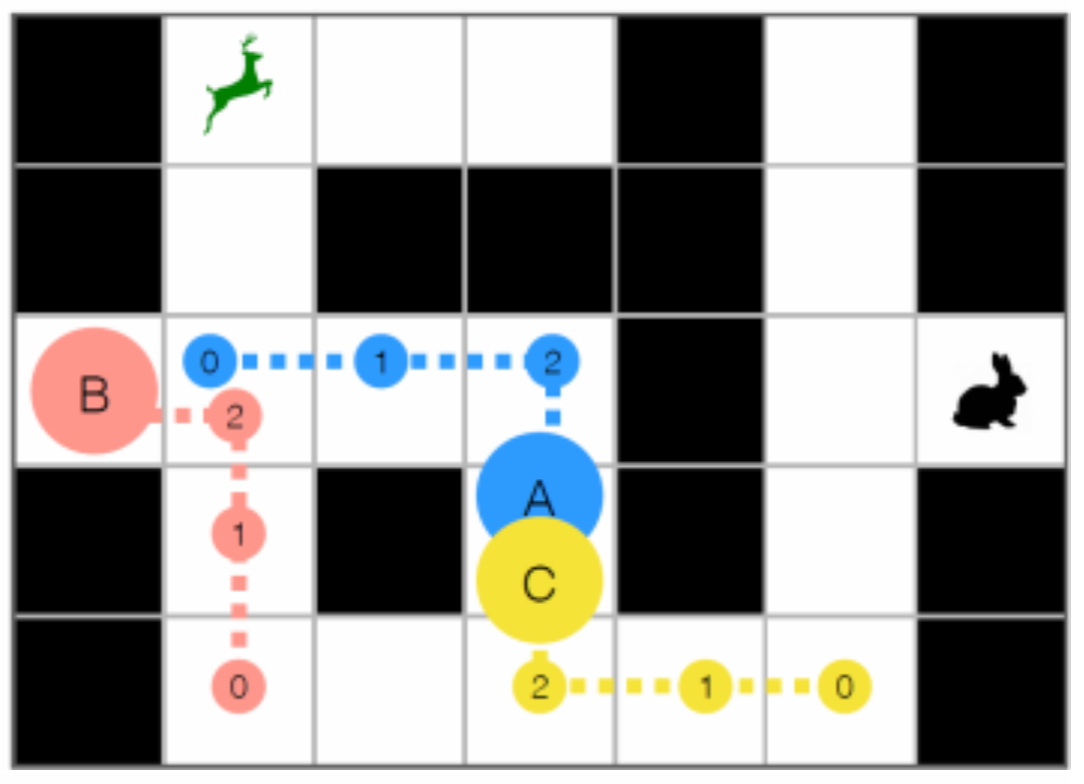
\includegraphics[width=0.75\linewidth]{Assets/scenario_one.png}
\vspace{0.5cm}
\caption{The first of nine stag-hunt scenarios. Circles represent hunters’ position at a given time step. Dotted lines represent motion. Figure adapted from Rabkina et al. (2019).}
\label{Figure:1}
\end{figure}

Figure \ref{Figure:1} is an example stag-hunt scenario \cite{Rabkina2019} where a pair of agents (A and B) cooperate to capture a stag and another agent captures a hare individually.
The circles represent a hunter's position at a given time-stamp and the dotted lines represent movement.
A key element of this game is the collaboration between agents which can be modeled using various methods.
One such method is a type of machine learning called Q-learning, which was used as the winning model in the Malmo Collaborative AI Challenge, hosted by Microsoft in 2017, a version of stag hunt where the agent was given two choices: 1) catch the pig by trapping it in a corner and receiving 25 points or 2) giving up and receive 5 points \cite{Katja2017}.
However, this solutions has limitations in how it could be extended beyond the Pig Chase task since the Q-learning model would need to be retrained for each new task, which is nontrivial, and that the secondary agent would choose either random actions or followed a heuristic search.
A rendering of the Malmo-Challenge environment can be seen in Figure \ref{Figure:2}.

Two of the solutions to these issues involved using a Bayesian model \cite{Shum2019} and Analogical Theory of Mind (AToM) \cite{Rabkina2019}, each of which will be discussed more in Section \ref{SectionTB}.
The AToM solution, which is the parent research project to this project, posited that AToM reasoning would allow agents to infer cooperation intentions of other agents and make predictions about other agents' future actions, leading to a model with a higher level of generalizability.
However, to test this data would need to be collected on the performance of that model in comparison to different implementations, such as a RL model.
This project aims to create a RL model for comparison for the AToM model using Q-learning with four additional factors to Pig Chase: 1) replacing the low-reward target of quitting with hares, 2) implementing the game with three hunters, two hares, and two stags, 3) the ability for the secondary agent to seek the low-reward targets and 4) using a 5x7 grid world.

These changes follow the spatial stag-hunt domain from Shum et al.'s model and allow a direct comparison between the two models, as well as data to be collected on human inference of the cooperation of agents.
In addition to the implementation of the Q-learning model, a reach-goal for the project is to gather data in a small study where participants would view episodes of the model playing stag hunt and inferring whether they perceive the agents cooperating together or not.

\section{Technical Background}
\label{SectionTB}

The implementation of the Q-learning model will be done with OpenAI's Gym environment, designed for "developing and comparing reinforcement learning algorithms." \cite{GymDocs, Brockman2016}
This environment provides a set of pre-made environments to reference as well as the ability to create a custom environment.
Since this Shum-style implementation is a grid-based environment with the only actions being movement in the four cardinal directions or staying in place , it will have a discrete observable- and action-spaces.
In the Shum et al. domain there are 9 maps that are used, so the observable-space will change depending on which map is chosen.
That set must be taken into account so that either the project uses a single map or a set of Q-learning models for different maps.
The action-space, however, will be consistent throughout each map.
Additionally, there were only time-steps in the implementation, which will remain true in the implementation of this project.

In reinforcement learning there are two main entities, the environment and the agent.
At first the agent takes some information about the current state of the environment, such as what is next to it.
The agent then decided on an action based on some strategy and receives a reward or penalty for that action.
The time that the agent receives the reward or penalty depends on the algorithm, but if it immediate and based on an estimate of the reward or penalty of the next state, like in this project, then it can be classified as a \textit{temporal difference methods}.
From this experience it learns to refine the strategy and iterates until it finds the optimal one.

In terms of a Q-learning model, a table of state and action pairs $(s, a)$ with an associated Q-value, representing their "quality," will be defined for each maps in the set.
Q-values are initialized to an arbitrary value and as the agent explores the environment they are updated.
The method for updating a Q-value consists of two parameters: $\alpha \in (0, 1]$ is the learning rate and $\gamma \in [0, 1]$ is the discount factor, which makes short-term or long-term rewards more valuable \cite{Kaelbling1996}.
The equation for this relationship can be written as \[ Q(s, a) = (1 - \alpha)Q(s, a) + \alpha(r + \gamma \text{max}Q_a(s', A)),\] where $r$ is the reward of an action, $s'$ is the next state, and $A$ is all the possible actions that can be taken \cite{}.
Additionally the algorithm uses $\epsilon$, which can be thought of the exploration parameter.
This tells the algorithm how often to pick a random action instead of the current most beneficial one from the Q-table.
In sum, we are learning the proper action by taking the old Q-value and adding the learned value of the immediate reward and possible future rewards.
This algorithm also has the potential to be optimized by modifying the values of the parameters either before or during training.
For example, the learning rate can be decreased as the knowledge base increases and the exploration parameter can be decreased as the number of trials increase.

The secondary agents will be implemented using a heuristic search algorithm, such as A-star.
The goal of these secondary agents are to mimic basic human-play, to some reasonable degree, to train the model to be able to cooperate with a human without require large amounts of human-play data, which would be infeasible to collect for this project.
The heuristic for these agents will operate around distance (e.g. distance of other hunters to targets, a hunters distance to a target compared to other hunters).

\section{Prior Work}

The two solutions touched on earlier aim to solve the problems of cooperation inference and action prediction in the game.
From the perspective of one agent, there are two questions to be answered: 1) are other agents trying to cooperate with me to catch a stag and 2) what behavior will they exhibit if they are/are not?
Shum et al.'s model is based on Bayesian inference with an explicit causal model, which map different behaviors to different states of the group of hunters.
Due to the explicit team hierarchy this model does not require training and was found to have strong correlations with human predictions in the experiments conducted to address the previous two questions.
Their contribution was a novel representation for extending single-agent generative models of action understanding to the to multi-agent interaction.
However, one of the limitations of this implementation is that it only works well for small groups, since as the number of agents grows the explicit team hierarchy also grows.

Alternatively, Rabkina et al. proposed a solution called Analogical Theory of Mind.
This process involves social reasoning called Theory of Mind \cite{Ruhl2020}, where an entity makes inferences about another’s mental state (knowledge, beliefs, preferences, desires, goals, and intentions).
The AToM model posits that a combination of analogical processes and feedback lead to the development of theory of mind reasoning without an underlying model of cooperation.
The AToM model is more accurate than the Bayesian model at most time stamps and does not require a predefined underlying hierarchy of team cooperation.
Furthermore, the ability to make predictions about the future actions of agents is an additional effect of reasoning about an agent’s cooperation with others.

% Malmo Challenge Environment Display {Figure 2}
\begin{figure}[ht]
\centering
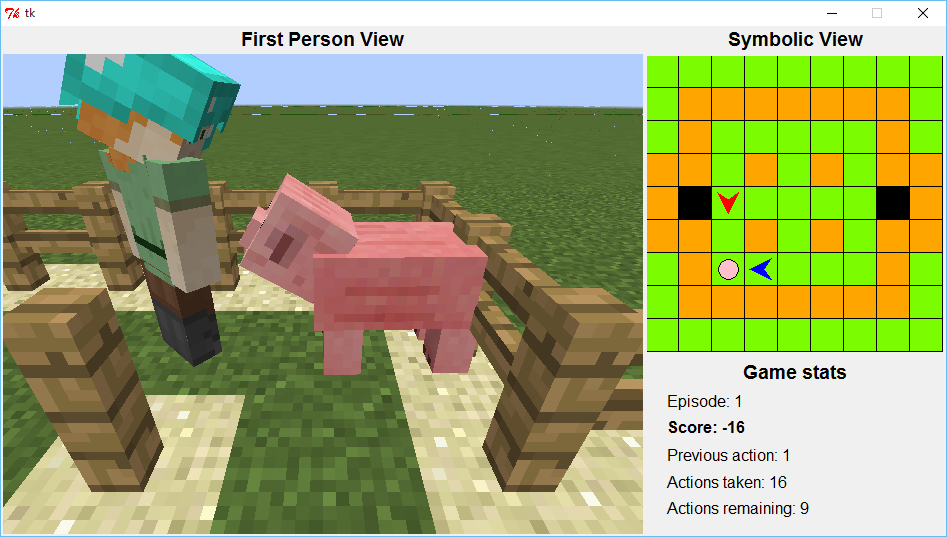
\includegraphics[width=0.75\linewidth]{Assets/pig-chase-overview.png}
\vspace{0.5cm}
\caption{Microsoft Malmo Platform PigChase environment. Left: actual 3D rendering in the Mamlo Platform. Right: symbolic representation of agent and pig on the map.}
\label{Figure:2}
\end{figure}

In addition to these models that utilize cognitive architectures for their reasoning, there are some models that use deep learning instead as part of the growing application of deep learning models in RL \cite{Nica2017}.
Arulkumaran et al. created a model that used the REINFORCE algorithm to create a 4 layer convolutional neural network \cite{Arulkumaran2017, Williams1992}.
They began by "pre-training" on an PigChase Replica Environment, a domain which approximated the Malmo-Challenge environment and was used to generate large batches of episodes for training.
Then they trained in the Malmo-Challenge environment using batches of 128 episodes and used the mean discounted return, for that particular time step in the game, as their evaluation metric.
Their resulting model was able to outperform a A-start heuristic, as expected, and solve the puzzle.
The significant question to consider from such a research project is the transferability of their model to different domains and how it's flexibility and performance compares to different models, such as Q-learning.

\section{Methods and Evaluation Metrics}

This project aims to create a RL mode for comparison for the AToM model of a Shum-style stag hunt game using Q-learning.
The first task is to create a custom environment using OpenAI Gym.
At this point I have complete a tutorial about using the Gym environment to create a Q-learning model for the taxi car problem \cite{Taxi-v3, Kansal2018}.
The observable space and action space for that problem and stag hunt have many similarities, the main difference in the action space being the pick-up and drop-off concepts in the taxi problem.

Luckily enough, the source code for the environment for this tutorial is public under an MIT License \cite{Taxi-v3Source}.
Meaning that I am able to view how OpenAI's team built their environment and modify it for my purposes.
To begin I am going to use the map that is seen in scenarios a, b, c, and h of Shum et al. Figure 2, also seen in Figure \ref{Figure:2} of this paper.
This observable space provides 20 positions so for hunters, stags, and hares we have 200, 160, and 40 possible states for each, respectively.
Thus in total there are 1,280,000 possible states for the Shum-style domain of that map, including trivial states (e.g. all hunters and targets generating at the same position.
Due to this large set of possibilities some measures may need to be taken to reduce this quantity if it proves too difficult to develop with, this may be where the Bletchly cluster becomes useful.
Additionally, development may need to move to a lower-level language than Python, such as C++, to increase computation speed.

A different issue that I need to deal with is the time I allow per episode.
In the Shum-style games, there were only three time-steps allowed before the episode finished.
Will this prove sufficient time for the model to learn or will this need to be compensated for by an increase in training episodes?
Part of my preparation will be adding a time constraint to the taxi problem and seeing the change in performance, then taking the insights I develop from there and apply them to this project.

For the secondary agents, I want to use an A-star algorithm in combination with some conditions.
My initial ideas involve determine which target to hunt by manhattan distance or value and then using the heuristic search to find the target.
Again, the space complexity of this algorithm becomes an issue but since the map isn't quite so large and the time allotted will be limited, I believe that this limitation is outweighed.
Moreover, when it comes to the behavior of the agents I will need to do research into what is the best way to represent basic human strategy in this game, while being consistent throughout each training episode.

\begin{table}[]
\caption{Example State-Indexed Q-Table: Each state has a list of Q-values that correspond to the action with same label as their index, e.g. at state zero action 0 has Q-value of 8.}
\vspace{0.2cm}
\center
\begin{tabular}{l|llllll|}
\cline{2-7}
                                             & \multicolumn{6}{c|}{action}                                                                                                                \\ \hline
\multicolumn{1}{|l|}{\multirow{6}{*}{state}} & \multicolumn{1}{l|}{}    & \multicolumn{1}{l|}{0}   & \multicolumn{1}{l|}{1}   & \multicolumn{1}{l|}{2}   & \multicolumn{1}{l|}{...} & m   \\ \cline{2-7} 
\multicolumn{1}{|l|}{}                       & \multicolumn{1}{l|}{0}   & \multicolumn{1}{l|}{8}   & \multicolumn{1}{l|}{3}   & \multicolumn{1}{l|}{2}   & \multicolumn{1}{l|}{...} & 4   \\ \cline{2-7} 
\multicolumn{1}{|l|}{}                       & \multicolumn{1}{l|}{1}   & \multicolumn{1}{l|}{-4}  & \multicolumn{1}{l|}{-7}  & \multicolumn{1}{l|}{-6}  & \multicolumn{1}{l|}{...} & 10  \\ \cline{2-7} 
\multicolumn{1}{|l|}{}                       & \multicolumn{1}{l|}{2}   & \multicolumn{1}{l|}{9}   & \multicolumn{1}{l|}{-8}  & \multicolumn{1}{l|}{-9}  & \multicolumn{1}{l|}{...} & -1  \\ \cline{2-7} 
\multicolumn{1}{|l|}{}                       & \multicolumn{1}{l|}{...} & \multicolumn{1}{l|}{...} & \multicolumn{1}{l|}{...} & \multicolumn{1}{l|}{...} & \multicolumn{1}{l|}{...} & ... \\ \cline{2-7} 
\multicolumn{1}{|l|}{}                       & \multicolumn{1}{l|}{n}   & \multicolumn{1}{l|}{5}   & \multicolumn{1}{l|}{7}   & \multicolumn{1}{l|}{-10} & \multicolumn{1}{l|}{...} & 1   \\ \hline
\end{tabular}
\end{table}

For the RL agent, this agent is currently thought to be implemented with the Q-learning algorithm but if the complexity of the project proves insufficient, then a more complex model will need to be used.
For now, a Q-learning model can be implemented with a Q-table in the Gym environment after the custom environment has been set up.
There is custom environment tutorial that I looked into \cite{Kathuria2021} and in combination with the Gym source code, setting up the custom environment seems to be within reasonable expectations.

\section{Ethical Considerations}

One of the main goals of the project is creating artificial agents with social reasoning, but to do that effectively and ethically we must reflect on what social contexts we are developing in.
These reflections start by analyzing the different value systems surrounding AI and its development \cite{Mohamed2020}.
Historically, the field has emphasized epistemic values and knowledge - prioritizing technical capabilities.
However, it has lacked the dedication to development with contextual values - the kind of values that can either challenge or perpetuate social inequalities.
As Mohamed et al. say, “the unique manner in which AI algorithms can quickly ingest, perpetuate, and legitimise forms of bias and harm represents a step change from previous technologies, warranting prompt reappraisal of these tools to ensure ethical and socially-beneficial use.”
There must be an increase in the priority of contextual values of these technologies or else we have a highly-capable tool with no social responsibility.
In the context of stag hunt, how might we develop the logic of the game to further encourage cooperation?
Is there a way to incentivize long-term cooperation instead of the short-term cooperation in the Shum-style game?
For example, in reality if two people work together, even if they fail, they might trust each other more as teammates and be more inclined to work together in the future.
There must be work done in the future to diversify the reward of social reasoning since it is so incredibly complex.

With the permeation of AI algorithms in our society and their ability to make such a massive impact on people in our society, it is instrumental that they hold the correct social goals in order to help society progress in the right direction rather than continue to devolve with traditional unjust values to marginalized groups.
Additionally, the decolonial AI theory considers those exploited at different levels by the algorithm - the ghost workers who organize the data to the beta-testers who test the algorithm. 
For this project, I find it essential to give credit wherever I can because even if something is given out freely the provider should get credit for their labor because the intentions that we put into a project shape the outcome of it.

The Voicing Erasure by the Algorithmic Justice League \cite{Koenecke2019, Koenecke2020} is a audio-visual art piece which discusses the racial disparities in algorithms, specifically speech recognition.
The piece begins to describe why pluralism is such a necessity by stating “Machines of silicon and steel that reflect the biases of their makers and their societies.”
These systems are created by human engineers, each of which has their personal set of biases and ignorances, so no system created can be truly neutral, as society currently views AI systems.
However, a neutral position is not a desirable one because it perpetuates the status quo - which thrives on the oppression of the poor, indigenous communities and communities of color.
In order to be a just system, it must take into account all biases present and not only work to avoid recreating them but also work to dismantle them, which is part of the important process of abolishment and reconstruction.
Even when these principles might not seem applicable it is essential that we consider them, such as in this project.
The development of agents being able to socially reason impacts the people that they reason with, so there are cultural, racial, sexual, religious, and more, considerations to make.
For example, how are the transitions between states being displayed?
Do they communicate the same intention to everyone or do the indicators bias certain groups that may be more familiar with specific physical signs?

As those who have been pushed to the periphery of our society come to the center, we must make sure to incorporate their perspective and experience into our technologies. Furthermore, their experience must not be exploited and reduced to mere data points but act as guiding forces to enhance the equitable reach of these algorithms - preventing the creation of future injustices and the continuation of current ones.
If the future development of these algorithms and ideas are going to work to increase the wellbeing of all groups of people, then we have to make sure that those people are represented in the design process.
One of the benefits of Q-learning is that the reward is given at each state transition so if something is going wrong a different strategy may be applied.
Similarly, it is important to incorporate a representative group of people in our design process in order to shift our strategy if we discover we are doing something wrong.

The representation of different users is one of the reasons that explainability is important.
Explainability is a framework that argues for the need for an AI system to explain the criteria and rubric for its decision making and its rationale.
In many cases, algorithms operate in a black box with know way to understand how they came to the conclusions they have.
With Q-learning, we have the weights to explain decisions but it is incredibly difficult to parse out how those weights were calculates when they may have been impacted by thousands, if not more, episodes.
Until we are able to have a level of control with AI where we can understand how exactly it got to the conclusion it did, one of the most important things we can do are make serious considerations about where we apply it.
There are problems that don't require AI or machine learning, but the buzz of the industry can lead to questionable products as a result of technological solutionism.
In this project the social reasoning is the most important ethical consideration we can make, while we do that through the design we can make sure that we operate ethically by giving credit, include as many kinds of users as possible in the design process, and reflecting on applications of our algorithms.

\section{Timeline}

The major preparatory step for this project is doing more research around reinforcement learning, especially in stag hunt.
So far there have been quite a few resources for both single and mult-agent stag-hunt using reinforcement learning so finding which algorithm will work best for this project will be key.
In the summer, after the Occidental College URC program begins, I plan to begin doing this research in tandem to my other role on the parent project.
Most of the summer will mainly consist of this research so that in the fall the project has a clear direction.
I want to be able to have a concrete understanding of the pros and cons of different models and have a series of goals to improve the project as it develops (e.g. user testing, optimizing parameters in the model).
In May I plan to learn more about the existing models of the project and how the new implementation may account for some gap in functionality or theory.
June will likely then be reserved for researching models I would want to build myself, which involves loosely designing the model I choose in terms of high-level implementation.
This phase of the project will be building the prior work that has been done in terms of stag-hunt, reinforcement learning, or multi-agent games.
In July I plan to continue designing the model and developing the kind of technical information I may need.
Additionally, this time period of high- to mid-level design would provide a good opportunity to start putting together a list of resources needed by the project, i.e. are there any computational tools I might need to request in the fall?

In the fall, I plan to start creating the custom environment and the agent models.
The semester starts in August so I would like to finish the design of the model in order to have it ready to implement in September.
I don't expect creating the custom environment to take a long time so I plan to finish that first since it's a prerequisite for the Q-learning model which I think will be the most difficult portion of the project.
This phase revolves around creating the specific methods I'm using in my implementation, such as the A-star and agent methods.
In September I plan to finish implementing the model and start trying to improve it, e.g. optimizing the parameters.
October will consist of evaluating the model and gaining insight into the performance of the model and how well it meets the goals of my comprehensive project and the parent project.
In November and December I want to conduct a small study for user testing to gather data on if and how people think the agents are cooperating.
Additionally, I will be preparing for my presentation and maybe trying to integrate with the parent project's docker system depending on the pace of the project.

\printbibliography

\end{document}
